%!TEX root = origin_elements_lecture_notes.tex

\chapter{Nucleosynthesis of Proton-rich Nuclei}

While neutron capture reactions can form most of the isotopes more massive than iron, isotopes that lie on the proton-rich side of the valley of stability were early on recognized to have another origin than neutron capture \citep{burbidge57,cameron57}. Originally it was believed that all of these isotopes formed by proton capture reactions in the so-called \emph{p}-process. Further studies have however shown that various different processes need to be invoked in order to produce proton-rich (\textit{p}-) nuclei. A classical ``\textit{p}-process'' does not exist and while the term \textit{p}-nuclei can be interpreted as \textit{p}roton-rich nuclei, it surely also stands for \textit{p}uzzling nuclei.

\section{Observations}\label{sec:p-nuclei:observations}

All \textit{p}-nuclei represent minor isotopes of their respective elements, meaning that no element is dominated by their \textit{p}-nuclei composition. Since astronomical observations mainly allow the determination of elemental abundances, the origin of \textit{p}-nuclei cannot be determined by spectroscopy. This leaves stardust (Chapter~\ref{ch:stardust}) and solar abundances (Chapter~\ref{ch:solar_system_abundances}) as the only observables to study the origin of the \textit{p}-nuclei.

The solar composition of \textit{p}-nuclei can be determined by fitting \ac{sproc} and \ac{rproc} models such that they can explain most of the isotopes in the Solar System. The proton-rich ``leftovers'', i.e., the \textit{p}-nuclei, then require another origin. Such approaches, see, e.g., \citet{bisterzo14}, have been fairly successful in defining the isotopes that lack a nucleosynthetic origin. Note though that for some nuclei, e.g., \ex{94}Mo, a mixed origin is possible. In this example, part of the \ex{94}Mo nucleus can be produced in the \ac{sproc}. The majority of its abundance however requires another origin.

Stardust grains can also significantly constrain the origin of certain \textit{p}-nuclei since measurements allow the determination of the abundance of these nuclei in the nucleosynthetic output of stars. So far, no clear \textit{p}-isotopic signature has been found in any individual stardust grain, which shows that either these sites are not sampled, or that the nucleosynthetic process forming \textit{p}-nuclei does not occur alone. For example, the stardust record might miss a nucleosynthetic site if it is either rare or does not produce dust. 
\begin{figure}[tb]
    \centering
    \includegraphics[width=0.75\textwidth]{graphics/p-nuclei/xenon-hl}
    \caption{Xenon isotopic composition for Xenon-HL composition, normed to \ex{132}Xe. See \citet{gilmour10} and references therein.}
    \label{fig:p-nuclei:xenon-HL_gilmour}
\end{figure}
One clear \textit{p}-nuclei related signature however is the so-called xenon-HL signature shown in Figure~\ref{fig:p-nuclei:xenon-HL_gilmour}. Here, the    isotopic ratios normed to \ex{132}Xe and normalized to the solar abundances are shown for all xenon isotopes. The so-called xenon-HL component, which is carried in presolar nanodiamonds, clearly shows in the heavy (H) and light (L) xenon isotopes as an overabundance compared to the solar composition, giving this component its name. It is unclear if the enrichment in heavy and light isotopes are correlated due to their nucleosynthetic origin, history, or not at all. Since xenon-HL is carried by nanodiamonds and only one in a million is expected to contain a single xenon atom, these samples can only be measured in bulk which makes a determination of the individual components impossible. Another interesting correlation between the \textit{p}- and \textit{r}-nuclei was recently found by \citet{stephan19}. These authors analyzed the molybdenum isotopic composition of SiC M grains, i.e., grains from \ac{agb} stars, with high precision using \ac{rims}. \citet{stephan19} used the fact that \ex{92}Mo is effectively destroyed in \ac{agb} stars to determine the precise molybdenum \ac{sproc} contribution. This further allowed these authors to also constrain the ratio of \textit{r}- to \textit{p}-nuclei, which appears to be constant for all analyzed stardust grains. This result indicates a common history of the molybdenum \textit{r}- and \textit{p}-nuclei, however, further measurements to solidify this finding are required.




\section{Nucleosynthesis processes}

With in-depth models of various nucleosynthetic processes, some of the classical \textit{p}-nuclei could be explained over the years. For \ex{164}Er, \ex{152}Gd, and \ex{180}Ta, a strong \ac{sproc} origin has been proposed, while \ex{113}In and \ex{115}Sn likely are produced jointly by the \ac{sproc} and \ac{rproc}. Furthermore, for \ex{138}La and \ex{180}Ta, a significant production originates likely from neutrino-induced reactions in \acp{sn}. In summary, this leaves the origin of 29 \textit{p}-nuclei to be explained.

\begin{figure}[tb]
    \centering
    \includegraphics[width=\textwidth]{graphics/p-nuclei/p-nuclei}
    \caption{Relative abundance of the \textit{p}-nuclei with respect to all \textit{p}-nuclei in the Solar System (blue) and to all isotopes of the respective element (orange).}
    \label{fig:p-nuclei:p-nuclei_abundance_relative}
\end{figure}
Figure~\ref{fig:p-nuclei:p-nuclei_abundance_relative} shows the relative abundance of each of these 29 \textit{p}-isotopes. The blue bars show the relative abundance with respect to the solar abundance sum of all \textit{p}-nuclei while the orange bars represent the relative abundance of each \textit{p}-isotope with respect to the element. Clearly, the most abundant \textit{p}-isotope is \ex{74}Se in the Solar System, followed by \ex{92,94}Mo,\ex{78}Kr, \ex{84}Sr, and \ex{96,98}Ru. All heavy \textit{p}-nuclei have very low abundance; in the Solar System and with respect to their parent element. This makes these isotopes especially difficult to detect and measure with high-precision in stardust grains, since these particles are very limited in size and therefore in the number of atoms they contain.

\begin{figure}[tb]
    \centering
    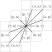
\includegraphics[width=0.5\textwidth]{graphics/p-nuclei/reaction_schematic}
    \caption{Overview of nuclear reactions that typically take place in stars.}
    \label{fig:p-nuclei:reaction_schematic_overview}
\end{figure}
An overview of nuclear reactions that typically take place in stars is given in Figure~\ref{fig:p-nuclei:reaction_schematic_overview}. The gray squares in the background indicate individual nuclei. As typical in context of the chart of the nuclides, the number of neutrons in the nucleus is plotted on the abscissa and the number of protons on the ordinate. Note that every reaction also has its reverse reactions, e.g., an $(n,\gamma)$ reaction can be reversed by a $(\gamma, n)$ reaction.

\subsection{\protect\boldmath The \texorpdfstring{$\gamma$}{gamma}-Process}
\begin{figure}[tb]
    \centering
    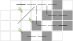
\includegraphics[width=0.6\textwidth]{graphics/p-nuclei/gamma_process}
    \caption{Schematic representation for the $\gamma$-process. Nuclei are schematically represented by boxes, as in the chart of the nuclides. Stable nucley are represented by gray filled boxes. Possible reactions that can take place are as shown in Figure~\ref{fig:p-nuclei:reaction_schematic_overview}.}
    \label{fig:p-nulcie:gamma_process}
\end{figure}
The $(\gamma, n)$ process creates proton-rich nuclei via photodisintegration reactions. A schematic of the $\gamma$-process in stars can be seen in Figure~\ref{fig:p-nulcie:gamma_process}. Potential reactions include the capture of photons and are shown in the schematic as labeled in Figure~\ref{fig:p-nuclei:reaction_schematic_overview}. These reactions all include the capture of a photon ($\gamma$), which is followed by the emission of a particle. In order to from a more proton-rich nucleus, potential particle emissions are neutrons, $\alpha$ particles, and protons, leading to the reactions $(\gamma, n)$, $(\gamma, \alpha)$, and $(\gamma, p)$, respectively. 

The $\gamma$-process is expected to occur at temperatures between $T_9 = 2$ to $T_9=3.5$ for only short amounts of time. This allows multiple photodisintegrations to take place in rapid succession. Depending on the conditions, nuclei far from the valley of stability can form on the proton-rich side. When nuclei reach the proton drip line, another photodisintegration cannot happen and the nucleus will undergo a $\beta^{+}$ decay, see box below. Once the event that created the $\gamma$-process in the first place passes, the unstable nuclei decay via $\beta^{+}$ decays along the isobars as indicated by green arrows in Figure~\ref{fig:p-nulcie:gamma_process}. This then leads to the production of proton-rich, stable nuclei.

\morebox{Proton drip line}{The proton drip is an line on the proton-rich side of the valley of stability. Beyond this line, i.e., on the more proton-rich side, nuclei will have a positive proton separation energy. Therefore, they become unstable and will decay via $\beta^{+}$ to remove one proton and turn it into a neutron via the reaction
\begin{equation}
    p \longrightarrow n + e^{+} + \nu_{e}.
\end{equation}
Here, a neutron, a positron $e^{+}$, and an electron neutrino are emitted.}

The curious reader might already have realized that the $\gamma$-process likely takes place in fast, explosive events, e.g., during a \ac{sn} explosion. Various potential astrophysical sites that could lead to the production of \textit{p}-nuclei are discussed below. However, they all have in common that the $\gamma$-process heavily depends on the seeds that are present, i.e., the available results of previous \ac{sproc} and \ac{rproc} nucleosynthesis. 


\subsection{The \textit{rp}-Process}

The \acf{rpproc} has been proposed to take place in very proton-rich environments. Charged particle reactions generally do not take place under normal conditions since the Coulomb barrier prevents nucleosynthesis. However, at temperatures $T_8 > 5$, these reactions can become frequent enough such that the \ac{rpproc} can take place, which leads to the synthesis of proton-rich nuclei.  Compared to the $\gamma$-process, the \ac{rpproc} is a primary process, which means that seeds are not required to explain the creation of proton-rich nuclei.

\begin{figure}[tb]
    \centering
    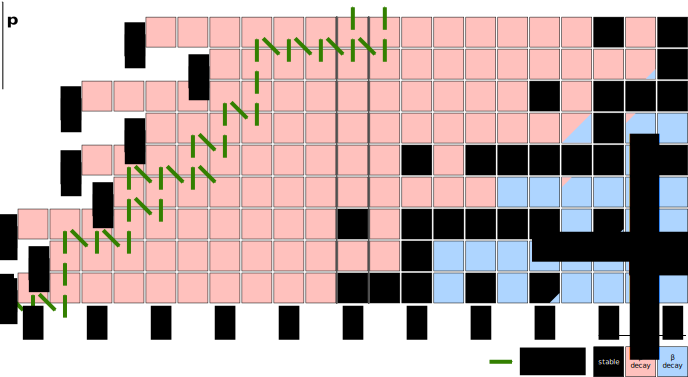
\includegraphics[width=\textwidth]{graphics/p-nuclei/rp-proc}
    \caption{A schematic of the path the \ac{rpproc} takes in the zirconium to cadmium region. Note that this region includes some of the most abundant \textit{p}-nuclei, namely \ex{92,94}Mo and \ex{96,98}Ru.}
    \label{fig:p-nuclei:rp-process}
\end{figure}
Figure~\ref{fig:p-nuclei:rp-process} shows the path the \ac{rpproc} takes in the region between zirconium and cadmium. Proton captures create heavier and heavier isotopes along the proton drip line, see above. The natural termination point of the \ac{rpproc} is reached at the neutron magic \ex{100}Sn. Subsequently, \ex{100}Sn decays via $\beta^{+}$-decay to \ex{100}Ru. The \ac{rpproc} can thus effectively create proton-rich isotopes up to ruthenium, i.e., the light and very abundant \textit{p}-nuclei.


\subsection{\protect\boldmath The \texorpdfstring{$\nu$}{nu}\textit{p}-Process}

In the $\nu$\textit{p}-process, protons can be produced by the reaction 
\begin{equation}
    \nu_e + n \longleftrightarrow  p + e^{-}. \label{eqn:p-nuclei:nu_capture_on_n}
\end{equation}
In this proton-rich matter, proton captures can lead to the formation of light \textit{p}-nuclei
However, depending on the exact stellar conditions, the reaction 
\begin{equation}
    \bar{\nu}_e + p \longleftrightarrow n + e^{+} \label{eqn:p-nuclei:nubar_capture_on_p}
\end{equation}
can also take place, leading to the production of neutron-rich areas.

Since neutrinos are directly involved in the creation of protons, this process was coined $\nu$\textit{p}-process. It has originally been proposed to take place in supernova explosions in the innermost zones right after the electron degeneracy is lifted.



\section{Astrophysical Sites}

\subsection{Core-collapse supernovae}

\paragraph{The $\gamma$-process}
Originally, the \textit{p}-process was proposed to take place in the outer ejecta layers of \acfp{ccsn}. While we know now that such a classical \textit{p}-process does not exist, many of the nuleosynthesis ways to create \textit{p}-nuclei still are expected to take place in these stellar events. Simulations of \acp{ccsn} in 1D show that the $\gamma$-process can take place when the \ac{sn} shock front passes through the O/Ne burning zone. The innermost part of this zone can reach peak temperatures and densities of $T_9=3.45$ and $7.85\times10^5$\,g\,cm$^{-3}$, respectively. These values drop in the outermost layers of the O/Ne burning zone to $T_9=1.79$ and $1.68\times10^5$\,g\,cm$^{-3}$, respectively. Under the hottest conditions, heavy \textit{p}-nuclei are actively destroyed and lighter ones are formed. This can be understood easily since such hot conditions allow photodisintegration of these heavy nuclei to proceed, see Figure~\ref{fig:p-nulcie:gamma_process}. At temperatures between 2.5\,GK and 3\,GK, intermediate mass \textit{p}-nuclei are significantly produced. Finally, the heavy \textit{p}-nuclei are produced at moderate temperatures below 2.5\,GK. 

Currently, $\gamma$-process models significantly underproduce the proton-rich isotopes \ex{92,94}Mo and \ex{96,98}Ru by more than one order of magnitude when other \textit{p}-nuclei are produced in the proper amounts. While these results are mostly independent of the initial mass of the \ac{ccsn} progenitor, they depend heavily on the original seed distribution. Furthermore, uncertainties in the explosion itself induces significant uncertainties in the $\gamma$-process yields. For example, the fallback parameterization in 1D \ac{ccsn} models might change significantly depending on the prescription used, which will thus change how much material can be recycled back into the galaxy after the \ac{sn} explosion. Since \textit{p}-nuclei cannot be observed directly but only in their aggregated state, e.g., as a part of the Solar System composition, detailed \ac{gce} models are generally required to study their exact origin. Such simulations allow us to understand the astrophysical impact of all adjustable parameters in the \ac{sn} models with respect to the origin of \textit{p}-nuclei. 

\paragraph{The $\nu$\textit{p}-process}
The $\nu$\textit{p}-process is thought take place in the inner ejecta of \acp{ccsn}. Models with accurate neutrino transport showed the existent of proton-rich areas under these conditions, as well as in the early wind from the protoneutron star. Large neutrino energy depositions first raise the energy, therefore lifting the electron degeneracy. This then allows the neutrino reactions shown in equations~\eqref{eqn:p-nuclei:nu_capture_on_n} and~\eqref{eqn:p-nuclei:nubar_capture_on_p} to proceed, which leads to the production of proton- and neutron-rich matter. The early models of \citet{frohlich06} showed that the $\nu$\textit{p}-process can lead to a significant increase of \ex{92,94}Mo and \ex{96,98}Ru under these conditions. More detailed models by \citet{bliss18} showed that neutrino-driven winds in \acp{ccsn} can indeed produce significant amounts of these isotopes, however, the production can at most explain the solar abundance of \ex{98}Ru. Their models however contribute $\lesssim40$\% of the solar \ex{96}Ru, $\lesssim27$\% of the solar \ex{92}Mo, and $\lesssim14$\% of the solar \ex{94}Mo. Another origin of these isotopes is thus required.



\subsection{Type-Ia Supernovae}

In addition to \acp{ccsn}, \acp{snia} have also been proposed as hosts of the $\gamma$-process. So far, mostly the single-degenerate scenario, in which the \ac{snia} explosion is initiated by a \ac{wd} reaching the Chandrasekhar mass limit by accreting matter from a companion star, has been investigated. Details on \acp{snia} can also be found in Section~\ref{sec:massive_stars:snia}. These scenarios have in fact been studied in 2D models by \citet{travaglio11}.
\begin{figure}[tb]
    \centering
    \includegraphics[width=\textwidth]{graphics/p-nuclei/snia_2d_models}
    \caption{2D models of \ac{snia} explosions including nucleosynthesis calculations. For details, see text. Temperature color coding for tracer particles are as following: Black: $T_9^\mathrm{peak} >7$, gray: $3.7 < T_9^\mathrm{peak} < 7$, red: $3< T_9^\mathrm{peak} < 3.7$, green: $2.4< T_9^\mathrm{peak} < 3$, blue: $1.5< T_9^\mathrm{peak} < 2.4$. \citet{travaglio11}, \copyright\ 2011 The American Astronomical Society.}
    \label{fig:p-nuclei:snia_2d_models}
\end{figure}
Figure~\ref{fig:p-nuclei:snia_2d_models} shows an excerpt of models by \citet{travaglio11}. The figures show snapshots of the star 0.8\,s (left) and 1.45\,s (right) after ignition. In each of these figures are shown the hydrodynamic evolution of the explosion (left) and the position of the Lagrangian tracer particles on the right. A minimal nuclear reaction rate network is used in order to calculate the hydrodynamic evolution of the star. This allows that the computational time for the shown 2D simulation to stay reasonable. Full nucleosynthesis calculations are subsequently performed by distributing so-called Lagrangian tracer particles into the hydrodynamics simulations. For each particle, the post-processing code follows its trajectory and determines the appropriate nucleosynthesis output. The locations of the tracer particles are shown on the right-hand sides in the figures above. Here, the particles are color-coded according to the peak temperature that they have experienced. Clearly some of these tracer particles have experienced high enough temperatures such that the $\gamma$-process can effectively take place. 

As for the \ac{ccsn} scenario, relevant $\gamma$-process nucleosynthesis in \acp{snia} only occurs if a prior \ac{sproc} enrichment exists. It is therefore essential to understand the distribution of these seeds that are obtained during the \ac{wd} accretion stage before reaching the Chandrasekhar mass. Consistent stellar calculations currently do not exist. Still, \ac{snia} models are likely significant contributors of \textit{p}-nuclei to the galaxy and efforts are underway to study in more detail the effect of the seed composition with respect to \textit{p}-nuclei production.

\subsection{X-Ray Bursters}

When a star in a binary system is sufficiently massive that it dies as a \ac{ccsn}, the remnant of these stars could either be a neutron star or a black hole. The neutron star can then, in certain cases, continue accreting mass from the companion star assuming that it has not been completely destroyed by the \ac{sn} and that the two stars are close enough. This donor star gives matter to an accretion disk around the neutron star, from which mostly hydrogen slowly falls in. Typical mass accretion rates are on the order of $10^{-8}\,M_\odot\,$a$^{-1}$ to $10^{-10}\,M_\odot\,$a$^{-1}$, while separation distances of the neutron and donor stars are 0.001\,AU to 1\,AU. These distances translate to orbital periods of around 0.01\,d to 100\,d. 

Once a hydrogen layer that is a few meters thick accumulates on top of the neutron star, a shell of hydrogen slowly begins to burn about a meter below the surface. About another meter further down, helium shell burning ignites as well. This fusion of helium is explosive and releases a total of around $10^{32}\,$J within a few seconds. The surface of the star in this event achieves a temperature of $T_7\approx 3$. According to Wien's displacement law as shown in equation~\eqref{eqn:solar_system_abundances:wiens_displacement_law}, the wavelength peak of such an event is approximately 100\,pm, which is in the X-ray part of the electromagnetic spectrum. Such \acp{xrb} have first been discovered in the late 1960s by Riccardo Giacconi, who received the Nobel Prize in Physics for this pioneering work in 2002.

During the \ac{xrb} event, temperatures in the shell exceed limits to activate the CNO and hot-CNO cycles to induce further nuclear burning. Once temperatures exceed around $T_8 \approx 5$, the reaction rate network can break out from the hot-CNO cycles and the \ac{rpproc} starts.

The \ac{rpproc} is very attractive since it naturally terminates at the neutron magic \ex{100}Sn and thus cannot produce nuclei heavier than ruthenium. This could, theoretically, explain why these light \textit{p}-nuclei with $A<100$ are more frequent in the Solar System compared to heavier ones, see Figure~\ref{fig:p-nuclei:p-nuclei_abundance_relative}. However, according to stellar simulations, the products that form in the \ac{rpproc} that takes place in X-ray bursters are not expected to be ejected. Thus, current simulations cannot account for these nuclei to be recycled back into the Milky Way.



% \subsection{Gamma-Ray Bursts}

% In the 1960s, the Vela series of military satellites were launched to check for compliance of the former Soviet Union with the 1963 nuclear test ban treaty. These satellites looked for $\gamma$-rays of terrestrial origin that would have originated from explosions of nuclear weapons. By 1967, military scientists had concluded that signals that were detected by these satellites did not come from the Earth below but rather from the stellar events above. This information was not disclosed to the public until 1973. 

% \acp{grb} happen around once per day in some random location in the sky. They last from around $10^{-2}$\,s up to $10^{3}$\,s and have very fast rise times of less than a tenth of a millisecond followed by an exponential decay of the signal. However, without knowing the distance to the origin of \acp{grb}, it was impossible to determine the processes that produced these events. The measured energy fluence for individual events ranges from $10^{-12}$\,J\,m$^{-2}$ up to $10^{-7}$\,J\,m$^{-2}$. In order to study \acp{grb}, the space shuttle Atlantis released on April 5, 1991, the \ac{cgro} in the Earth's orbit. Several massive bursts were recorded by \ac{cgro}, among which are a burst with a peak photon energy of 18\,GeV on December 15, 1994, which lasted for 90\,min. 

% Ultimately, the successful combination of \ac{grb}-event detection in space with optical follow-up observations showed that \acp{grb} are of extragalactic origin. In fact, as for \acp{sn}, \acp{grb} are also dividable into two classed. Events that last longer than two seconds are referred to as long-soft \acp{grb} and are likely associated with \acp{sn}. Shorter events on the other hand are called short-hard \acp{grb} and seem to be associated with \ac{ns}-\ac{ns} or \ac{ns}-\ac{bh} mergers.

% \textcolor{red}{Where does the rp process take place and how? -> It doesn't, but it takes place in \acp{xrb}!!!}



\section{Puzzling Nuclei}

The origin of the \textit{p}-nuclei clearly remains \textit{p}uzzling. One of the main factors hindering our understanding of the astrophysical sites is that no element is dominated by a \textit{p}-isotope. Therefore, astronomical observations cannot currently detect a hypothetical \textit{p}-rich ejecta from a star since spectroscopic observations are not sensitive enough to individual isotopes. The Solar System abundances, see Chapter~\ref{ch:solar_system_abundances}, are, along with stardust grains, among the sole observations that can be used to decipher the origin of the proton-rich isotopes. While no stardust grain that shows a clear \textit{p}-nuclei isotopic pattern has been found yet, a recent high-precision \ac{rims} study \citep{stephan19} has shown an indication that the \textit{p}-nuclei might be correlated to the \ac{rproc} nuclei, at least for molybdenum. Earlier xenon measurements, especially the occurrence of the Xe-HL component as shown in Figure~\ref{fig:p-nuclei:xenon-HL_gilmour} allows for further speculations of such a common origin. Clearly, more measurements are required and are currently ongoing. Hopefully, stardust grain measurements can in the near future help to better understand the origin of the \textit{p}-nuclei.

The theoretical front is also continuously pushed towards optimizing model predictions to better understand the formation of these nuclei. As pointed out multiple times, the seed nuclei distribution, i.e., the nuclei that are produced in the \ac{sproc} prior in \acp{sn} prior to explosion, need to be better constrained since their abundance significantly influences the production of proton-rich isotopes in the $\gamma$-process. Furthermore, a better and more detailed understanding of \acp{snia} models and the exact scenario under which these explosions take place (single versus double-degenerate precursors) will also constrain these objects as potentially significant contributors to the $\gamma$-process. While the critical reaction rates for \textit{p}-nuclei formation have been studied in the framework of a 1D \ac{sn} model for a $25\,M_\odot$ star \citep{rauscher16}, such sensitivity studies should be extended to other potential astrophysical sites that could explain \textit{p}-nuclei formation. Furthermore, future experiments will hopefully allow us to directly measure the critical reaction rates. 

Finally, to establish a coherent picture of \textit{p}-nuclei formation in the Milky Way, accurate \ac{gce} model are crucial. While most of these models focus on constraining \ac{gce} for the elements in the Milky Way, constraints for the evolution of isotopes are slowly coming together. Specific isotope constraints will ultimately be of key importance in order to consider \textit{p}-nuclei formation from various different sources. Here, stardust grain measurements of various isotopes can help to improve \ac{gce} models since these measurements allow us to directly analyze the isotopic provenance of isotopes in the solar neighborhood prior to Solar System formation. Improvement in this area are currently under active investigation.